\section{Web Data Inspector}
\label{sec:web-data-inspector}

Web Data is composed of a colourful panel of datasets, coming from a variety of sources. Some datasets are created by integrating others. Datasets expose links between them in order to improve their connectivity to the rest of the data, thus allowing more relevant information to be accessible. As a user trying to retrieve some information from this heterogeneous collection of datasets, it is necessary to have sufficient insight into the dataset of interest so to formulate queries: the user need to understand how the data is structured, how a dataset is connected to others, and to assess in some way the quality of the data.

In this section, we present the \emph{Web Data Inspector} as a tool for inspecting the edges of a dataset though the use of graph summaries.

\subsection{Views into a Dataset}

Based on the graph summary, the Web Data Inspector presents various views of a dataset. This tool is part of the Sindice~\cite{oren:2008:sdl} project; its home page, shown in Figure~\ref{fig:wdi:home-page}, provides the user with a text box where he can enter the dataset's name of interest --- here, the domain name of the web site. By clicking the ``Check'' button he will be provided with several views useful in exploring the content and the structure of the chosen dataset.

Also, from the home page, the user has the possibility to choose an RDF class or an RDF property and then, upon clicking the ``Check'' button he will be shown the provenance datasets of such RDF element (classes or properties) as well as its relationships with other RDF elements.

\begin{figure}
	\centering
	\resizebox{.9\textwidth}{!}{
		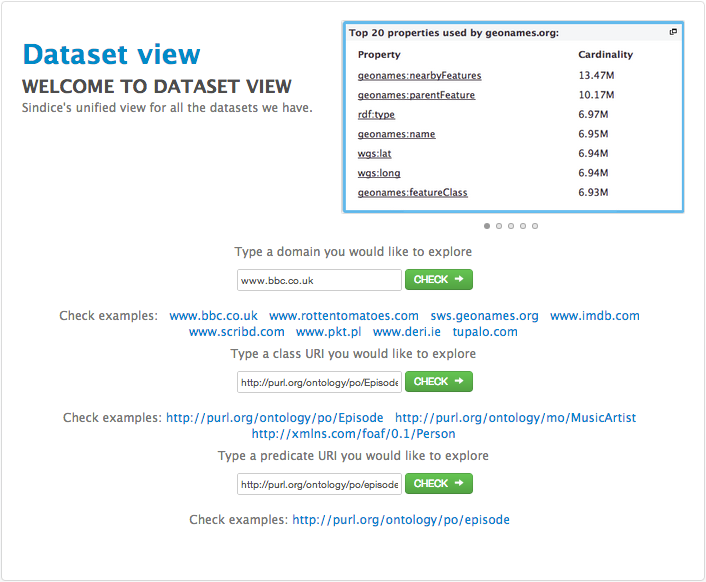
\includegraphics[scale=1]{exploiting/wlv/images/home-page}
	}
	\caption{Web Data Inspector - home page}
	\label{fig:wdi:home-page}
\end{figure}

In the next subsections, we will describe in more detail the different views that the user is provided with when exploring a dataset using the Web Data Inspector. 

\subsubsection{General View}

The general view tab as depicted in Figure~\ref{fig:wdi:generalView} shows a summary of some of the particular dataset's properties and statistics. This includes the domain address of the dataset and the size in terms of triples and documents. Further details and analysis is found in the other tabbed sections: ``Inside this dataset'', ``To/from datasets'', and ``Third party''.

\begin{figure}
	\centering
	\resizebox{.9\textwidth}{!}{
		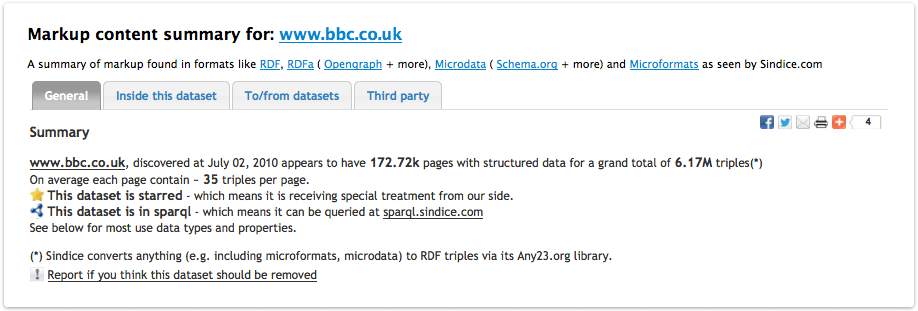
\includegraphics[scale=1]{exploiting/wlv/images/general.png}
	}
	\caption{Web Data Inspector - general view}
	\label{fig:wdi:generalView}
\end{figure}

\subsubsection{Inside This Dataset}

The ``Inside this dataset'' tab as depicted in Figure~\ref{fig:wdi:insideThisDataset} delves deeper into the dataset to explore and present information about the RDF properties and classes used within. This view shows the links that are classified as internal only to the dataset. From this view, you can learn more about the structure and content of the dataset.

\begin{figure}
	\centering
	\resizebox{\textwidth}{!}{
		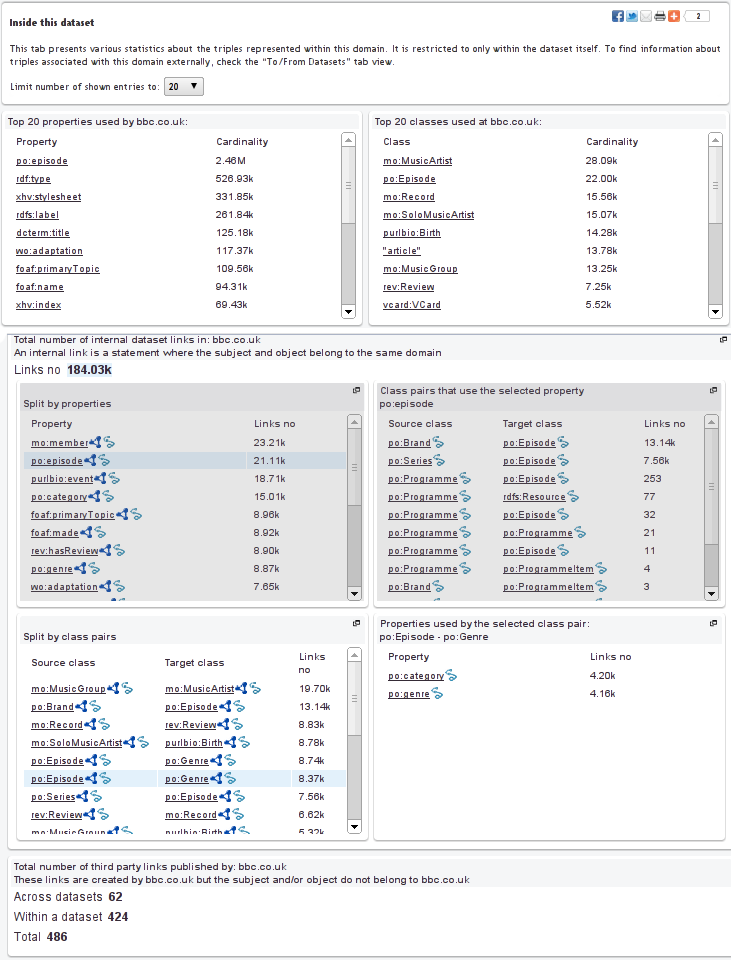
\includegraphics[scale=1]{exploiting/wlv/images/insideThisDataset.png}
	}
	\caption{Web Data Inspector - inside this dataset}
	\label{fig:wdi:insideThisDataset}
\end{figure}


\subsubsection{To/From This Dataset}

The ``To/from datasets'' tab as depicted in Figure~\ref{fig:wdi:toFromThisDataset} presents the existing links or relationships this dataset has with other datasets. From here, exploration can span across the many domains that the particular dataset is linked with.

\begin{figure}
	\centering
	\resizebox{\textwidth}{!}{
		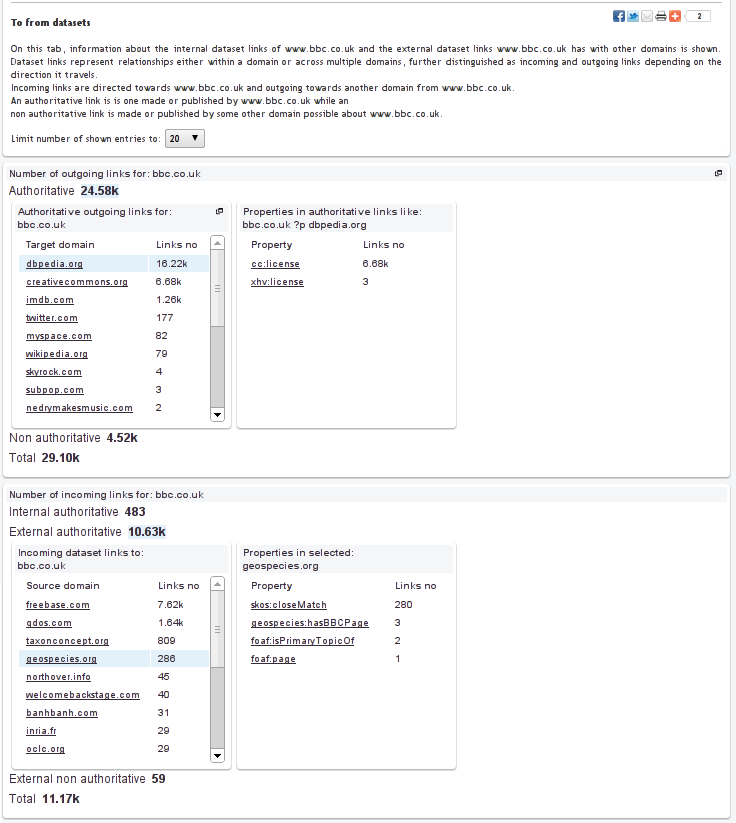
\includegraphics[scale=1]{exploiting/wlv/images/toFromDataset}
	}
	\caption{Web Data Inspector - to/from this dataset}
	\label{fig:wdi:toFromThisDataset}
\end{figure}

\subsubsection{Third-Party Links}

In regards to validating datasets, edge authority as defined in Defintion~(\ref{def:edge-authority}) helps dataset owners to distinguish another important aspect: third-party links. These represent links that do not have authority (non-authoritative); knowing such links is useful to discover if they that are incorrect or specify relationships that the owner does not explicitly agree with. In some cases, these links can be connotative to the idea of e-mail spam.

The ``Third-party links'' tab as depicted in Figure~\ref{fig:wdi:thirdPartyLinks} shows the user information about particular links that have been classified as non-authoritative by the graph summary.

\begin{figure}
	\centering
	\resizebox{.9\textwidth}{!}{
		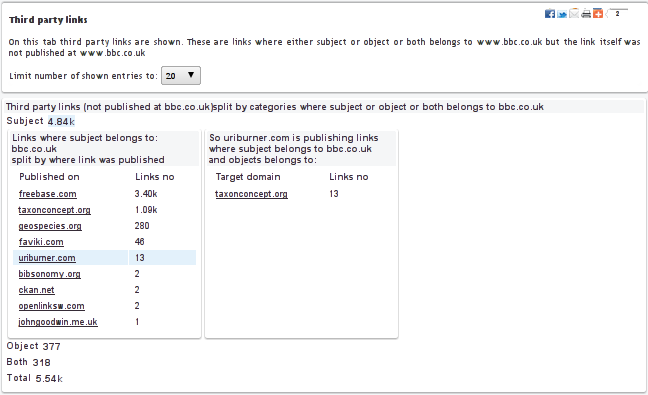
\includegraphics[scale=1]{exploiting/wlv/images/thirdPartyLinks}
	}
	\caption{Web Data Inspector - third party links view}
	\label{fig:wdi:thirdPartyLinks}
\end{figure}

\subsection{Evaluation}

In this section, we show how the Web Data Inspector tool works across some notable datasets: \textbf{bbc.co.uk}, \textbf{sws.gonames.org}, and \textbf{www.rottentomatoes.com}.

\subsubsection{bbc.co.uk}

The dataset ``bbc.co.uk'' uses RDFa to annotate their ``Programmes'' and ``Music'' websites. As depicted in Figure~\ref{fig:wdi:generalView}, there are over 6M triples that cover brands, series (seasons), episodes, artists, broadcast events, broadcast services, etc. The top 3 most used classes in the ``bbc.co.uk'' dataset are: ``article'' which appears 44.12K times, ``mo:MusicArtist'' 24.18K times and ``vcard:Name'' 20.48K times. The top 3 most popular properties are ``po:episode'' with 2.67M, ``rdfs:label'' with 216.78K and ``wo:adaptation'' with 139.14K, as depicted in Figure~\ref{fig:wdi:insideThisDataset}.

The ``bbc.co.uk'' dataset includes links to further URIs, allowing you to discover more data, e.g. about members of a band or about a certain series episode. It also includes a ``owl:sameAs'' link with 21.61K occurences to the corresponding DBpedia resource, allowing you to aggregate more data about that band, extracted from Wikipedia's infoboxes. From the ``To/from dataset'' view we see there are about 3K links that link ``bbc.co.uk'' to well known datasets like ``dbpedia.org'', ``myspace.com'', and ``imdb.com'' as reported by the ``outgoing links'' box. On the incoming links side, we see that not too many datasets are linked to ``bbc.co.uk'' as there are only 275 links that link other datasets like ``freebase.com'' and ``dbpedia.org'' to ``bbc.co.uk''.

\subsubsection{sws.geonames.org}

The dataset ``sws.geonames.org'' is a dump dataset rather than a website which provides over 129M triples, as depicted in Figure~\ref{fig:wdi:generalView}, about all countries and various geographical locations. Here we can find classes such as ``geonames:Feature'' which appears 7.85M times, ``wgs:Point'' 4.36K times and ``foaf:Agent'' with 2.41K occurences and properties such as ``geonames:nearbyFeatures'' with 14.28M occurences, ``geonames:name'' with 7.89M occurences and ``geonames:parentFeature'' with 7.88M occurences.

The ``sws.geonames.org'' dataset includes over 4M links to resources from other datasets like ``identi.ca'', ``nytimes.com'', or ``dbpedia.org'' as depicted by the outgoing links box in Figure~\ref{fig:wdi:toFromThisDataset}. This dataset is also well linked to by other datsets like ``naplesplus.us'', ``dbpedia.org'' or ``geospecies.org'' with over 274K incoming links.

\subsubsection{www.rottentomatoes.com}

Rotten Tomatoes is a film review aggregator which provides reviews, information, and news of films. It contains over 11M triples, as depicted in Figure~\ref{fig:wdi:generalView}, and it uses various proprietary vocabularies. Among the most popular classes we note ``actor'' which appears 147.19K times, ``sorg:Person'' 31.00K times, ``sorg:AggregateRating'' 2.94K times and ``video.movie'' 2.77K times.

The linkage for this dataset is very poor and we see that by the number 0 for the outgoing/incoming links box in Figure~\ref{fig:wdi:toFromThisDataset}. A possible improvement of the dataset might be the increase of the linkage of the dataset with links to well known datasets like ``dbpedia.org'' or specific datasets like ``imdb.com''.

\subsection{How to improve your dataset with the Web Data Inspector}

In this section we show how the results of the Web Data Inspector can be used as suggestions for improving one's dataset. Being able to see the classes and the properties of his dataset, the dataset owner is able to have a deep understanding of his dataset. He can determine if the dataset graph looks as planned.

For example, we may assume that the dataset contains the ``foaf:Person'' class which has, among others, the ``foaf:name'' and ``foaf:homepage'' properties. From the number of the occurences of these properties, the dataset owner can decide if his dataset is as he intended too: if he knows that most of the people in the dataset should have a homepage, then this should be reflected in similar numbers for the occurences of the ``foaf:name'' and ``foaf:homepage'' properties.

Also, the dataset owner can identify possible mistakes such as typos in the classes/properties names. For example, it is well known that ``foaf:name'' is a property of the FOAF vocabulary but ``foaf:naem'' is not.
